\documentclass{standalone}

\usepackage{tikz}

\begin{document}

    % Inspired by Stackoverflow answers at:
    % https://tex.stackexchange.com/questions/132321/generate-analog-clock-with-numbered-face
    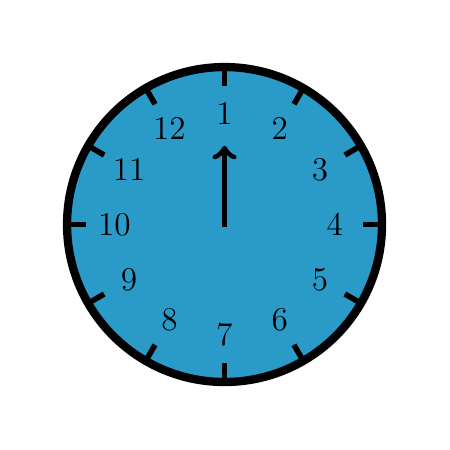
\begin{tikzpicture} [line cap=rect, line width=3pt]
        \node [shape=rectangle, minimum width=5cm, minimum height=5cm, anchor=center] at (0, 0) {};
        \filldraw [fill=cyan!80!black] (0, 0) circle [radius=2cm];
        \foreach \angle [count=\xi] in {90,60,...,-240}
        {
            \node [font=\large] at (\angle:1.4cm) {\xi};
            \draw [line width=2pt] (\angle:1.8cm) -- (\angle:2cm);
        }
        \draw [line width=2pt, ->] (0, 0) -- (90:1cm);
    \end{tikzpicture}

\end{document}